% ==============================================================================
% TCC - Nome do Aluno
% Capítulo 2 - Revisão da Literatura
% ==============================================================================
\chapter{Revisão da Literatura}
\label{sec-literatura}

Neste capítulo é feita uma revisão dos principais conceitos utilizados neste
trabalho, além de apresentar fundamentos para uma compreensão mais profunda dos
mesmos.

\section{Redes Neurais Feedfoward}

O primeiro conceito a ser compreender são as redes neurais \textit{feedfoward},
também conhecidas como \textit{perceptrons} de multiplas camadas, do inglês,
\textit{multitayer perceptrons} (\textit{MLP}). Redes \textit{feedfoward} 
podem ser entendidos como um modelo que simula o funcionamento de um cerebro,
em que os neurõnios formam um rede de conexões, em que o processamento se dá
pela passagem de informação por essa rede considerando a topologia, ou seja, as
conexões sinápticas entre os neurõnios e força des mesmas. Sendo que a força
pode ser de ativação (positiva), ou de inibição (negativa).
Nesta analogia, um neurõnio é entendido como uma unidade de processamento que 
ao receber estimulos de outros neurõnios, processa estas entradas e 
produz uma saída. Esta estrutura de neurõnio artificial foi proposta em 
\cite{mcculloch-pitts:1943-perceptron} e está esquematizada na figura 
\ref{fig:neuronio-de-pitts}.  

\begin{figure}[htpb]
\centering
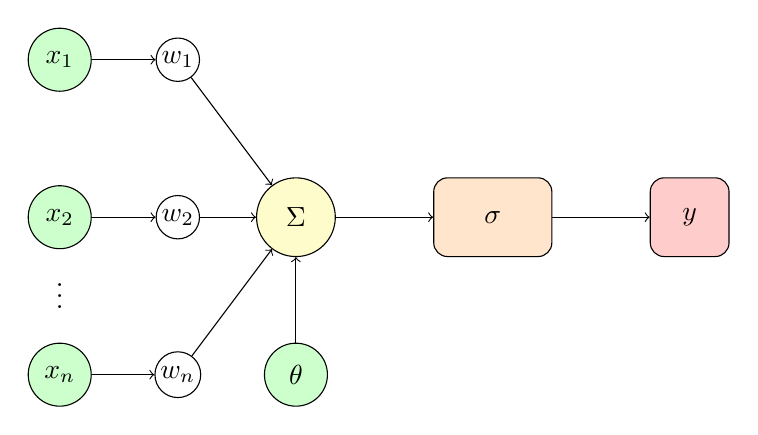
\begin{tikzpicture}[
    neuron/.style={circle, draw=black, fill=blue!20, minimum size=1.2cm},
    input/.style={circle, draw=black, fill=green!20, minimum size=0.8cm},
    weight/.style={fill=white, circle, draw=black, inner sep=1pt},
    arrow/.style={-Stealth, semithick},
    label/.style={text width=2cm, align=center, font=\small\sffamily}
]

\node[input] (x1) at (-3, 2) {$x_1$};
\node[input] (x2) at (-3, 0) {$x_2$};
\node at (-3, -0.9) {$\vdots$};
\node[input] (xn) at (-3, -2) {$x_n$};

\node[weight] (w1) at (-1.5, 2) {$w_1$};
\node[weight] (w2) at (-1.5, 0) {$w_2$};
\node[weight] (wn) at (-1.5, -2) {$w_n$};

\node[draw, circle, minimum size=1cm, fill=yellow!20] (sum) at (0, 0) {$\Sigma$};
\node[draw, rectangle, rounded corners=5pt, minimum width=1.5cm, minimum height=1cm, fill=orange!20] (act) at (2.5, 0) {$\sigma$};
\node[draw, rectangle, rounded corners=5pt, minimum width=1cm, minimum height=1cm, fill=red!20] (out) at (5, 0) {$y$};
\node[input] (b) at (0, -2) {$\theta$};

\draw (x1) edge[->] (w1);
\draw (x2) edge[->] (w2);
\draw (xn) edge[->] (wn);

\draw (w1) edge[->] (sum);
\draw (w2) edge[->] (sum);
\draw (wn) edge[->] (sum);

\draw (b) edge[->] (sum);
\draw (sum) edge[->] (act);
\draw (act) edge[->] (out);

\end{tikzpicture}
\caption{Representação gráfica de um neurónio de MacCough-Pitts. Fonte: elaborada pelos autores.}
\label{fig:neuronio-de-pitts}
\end{figure}

Formalizando matemáticamente a figura \ref{fig:neuronio-de-pitts},
sendo $W$ um vetor de pesos $\in [-1, 1]$, $\boldsymbol{x}$ um vetor de entradas
de tamanho $n$ e pertecente a $R^n$, $\theta$ um valor pertecente a $R$ 
e $\sigma$ uma função não linear. Um neurõnio é uma função $f: R^n -> R$,

\begin{eqnarray}\label{eq:neuronio-pitts}
    \sigma((\sum_{i=1}^{n} W_i\boldsymbol{x_i}) + \theta)
\end{eqnarray}

O termo $\theta$ pode ser entendido como o último elemento de $\boldsymbol{x}$ 
que está sendo sempre multiplicado pelo último elemento de $W$
que sempre tem valor igual a $1$, logo a equação \ref{eq:neuronio-pitts}
pode ser simplicada como,

\begin{eqnarray}\label{eq:neuronio-pitts-simplificado}
    \sigma(W\boldsymbol{x})
\end{eqnarray}

Um neurõnio pode ser entendido como uma transformação linear, a multiplicação
das entradas pelos pesos e viéses somados, seguida por uma
transformação não linear. Esta é feita pela função de ativação $\sigma$.
Alguns exemplos de funções de ativação empregradas nas redes neurais são A
função \textit{sigmoid} \ref{eq:sigmoid}, 
tangente hiperbólica (\textit{tanh}) \ref{eq:tanh}e 
\textit{Rectfied Linear Unit} (\textit{ReLU}) \ref{eq:relu}.

\begin{eqnarray}
    sigmoid(x) = \frac{e^x}{e^x}\label{eq:sigmoid}
    \\
    tanh(x) = \frac{e^x}{e^x}\label{eq:tanh}
    \\ 
    ReLU(x) = \frac{e^x}{e^x}\label{eq:relu}
\end{eqnarray}

Um único neurõnio não é capaz de aproximar qualquer função, para isso, eles são 
organizados em camadas que a saída de cada neurõnio de uma camada forma 
parte da entrada de todos os neurõnios da camada seguinte. 
A primeira camada apenas representa os dados de entrada, a última camada
representa um vetor de saída de tamanho 
Logo, uma rede neural \textit{feedfoward} com $L$ camadas escondidas 
pode ser entendida como uma função composta $f$ formada por 
um conjunto de consecutivas transformações lineares e não lineares num 
vetor de dados de entrada de tamanho $n$ $\boldsymbol{x} \in R^n$
que produz como saída um vetor de tamanho $m$ $\boldsymbol{\hat{y}} \in R^m$,  
sendo as transformações intermediárias representadas pelas saídas $y^l$ 
da camada escondida $l$, $l \in [1,..,L]$,

\begin{equation}\label{eq:rede-neural-composta}
    f(\boldsymbol{x}) = \sigma^{L + 1} y^{L + 1} \circ \sigma^{L} \circ y^{L} 
    \dots \circ \sigma^{2} \circ y^{2} \circ \sigma^{1} \circ y^{1}
\end{equation}

A figura \ref{fig:feedfoward-representacao-grafica} resume graficamente a
definição presente na equação \ref{eq:rede-neural-composta}.

\begin{figure}[htpb]
\centering
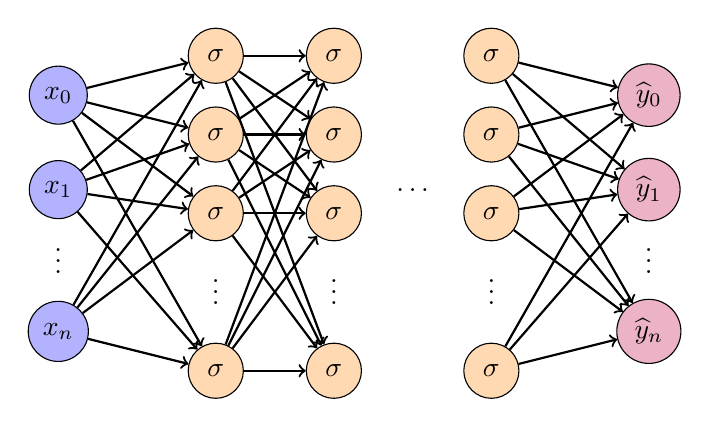
\begin{tikzpicture}[
    neuron/.style={circle, draw, minimum size=0.7cm},
    layer/.style={rectangle, minimum width=1.5cm, minimum height=8cm, draw=black, fill=blue!10, rounded corners=3pt},
    input/.style={neuron, fill=blue!30},
    hidden/.style={neuron, fill=orange!30},
    output/.style={neuron, fill=purple!30},
    physnode/.style={rectangle, draw, rounded corners, fill=orange!30, minimum width=1.5cm, minimum height=1.8cm},
    lossnode/.style={rectangle, draw, rounded corners, fill=yellow!30, minimum width=2cm, minimum height=3.2cm, align=center},
    every edge/.style={draw, ->, thick}
]

\node[input] (I-1) at (0, 3.5) {$x_0$};
\node[input] (I-2) at (0, 2.3) {$x_1$};
\node at (0, 1.5) {$\vdots$};
\node[input] (I-3) at (0, 0.5) {$x_n$};

\node[hidden] (H1-1) at (2, 4) {$\sigma$};
\node[hidden] (H1-2) at (2, 3) {$\sigma$};
\node[hidden] (H1-3) at (2, 2) {$\sigma$};
\node at (2, 1.1) {$\vdots$};
\node[hidden] (H1-4) at (2, 0) {$\sigma$};

\node[hidden] (H2-1) at (3.5, 4) {$\sigma$};
\node[hidden] (H2-2) at (3.5, 3) {$\sigma$};
\node[hidden] (H2-3) at (3.5, 2) {$\sigma$};
\node at (3.5, 1.1) {$\vdots$};
\node[hidden] (H2-4) at (3.5, 0) {$\sigma$};

\node at (4.5, 2.3) {$\dots$};

\node[hidden] (Hn-1) at (5.5, 4) {$\sigma$};
\node[hidden] (Hn-2) at (5.5, 3) {$\sigma$};
\node[hidden] (Hn-3) at (5.5, 2) {$\sigma$};
\node at (5.5, 1.1) {$\vdots$};
\node[hidden] (Hn-4) at (5.5, 0) {$\sigma$};

\node[output] (O-1) at (7.5, 3.5) {$\widehat{y}_0$};
\node[output] (O-2) at (7.5, 2.3) {$\widehat{y}_1$};
\node at (7.5, 1.5) {$\vdots$};
\node[output] (O-3) at (7.5, 0.5) {$\widehat{y}_n$};

% Connections
\foreach \i in {1,2,3}
    \foreach \j in {1,...,4}
        \path (I-\i) edge (H1-\j);

\foreach \i in {1,...,4}
    \foreach \j in {1,...,4}
        \path (H1-\i) edge (H2-\j);

\foreach \i in {1,...,4}
    \foreach \j in {1,...,3}
        \path (Hn-\i) edge (O-\j);

\end{tikzpicture}
\caption{Representação gráfica das redes \textit{feedfoward}. Fonte: elaborada pelos autores.}
\label{fig:feedfoward-representacao-grafica}
\end{figure}

O vetor de saída $\boldsymbol{\hat{y}}$ é então comparado com um vetor desejado 
$\boldsymbol{y}$ para calcular o erro entre a saída da rede e a saída desejada.
Este é o papel da função de perda (\textit{loss function}). 
Usualmente, para o caso de uma regressão, emprega-se a função de erro quadrático médio, 
do inglês, \textit{mean root square} (\textit{MSE}), como definida na equação
\ref{eq:mse}.

\begin{equation}\label{eq:mse}
    MSE = \frac{1}{N} \sum_{i=0}^{N}(y_i - \hat{y}_i)^{2}
\end{equation}

A atualização dos pesos de cada camada se dá pela cálculo do grandiente
de uma função de erro $\mathcal{L}$. O "tamanho do passo" que será dado
é determinado por um parâmetro $\alpha$ chamado de taxa de aprendizagem.

\begin{eqnarray}\label{eq:atualizacao-parametros-redes}
    W_i^{t + 1} = W_i^{t} + \alpha \nabla \mathcal{L}
\end{eqnarray}

A propagação dos erros se dá pelo algoritmo de retropropagação, sendo um caso 
de aplicação da regra da cadeia. 


\section{Redes Neurais Informadas pela Física}

Apresentadas em \cite{raissi-etal:19}, PINNs podem ser entendidas como uma forma
avançada de regularização, ou como um problema de otimização que transforma 
as condições de fronteira e iniciais em penalizações para a função custo. PINNs
são capazes de resolver problemas no seguinte formato: 

\begin{eqnarray}
    \mathcal{D}(u(\boldsymbol{x},t);\boldsymbol{\lambda}) &=& f(u,\boldsymbol{x},t), \quad \boldsymbol{x} \in \Omega, \, t \in I, \label{model-1-a}\\
    %
    \mathcal{B}(u(\boldsymbol{x},t)) &=& g(\boldsymbol{x},t), \quad \boldsymbol{x} \in \Gamma, \, t \in I, \label{model-1-b}\\
    %
    \mathcal{I}(u(\boldsymbol{x},t_0)) &=& q(\boldsymbol{x}), \quad \boldsymbol{x} \in \Omega, \label{model-1-c}
\end{eqnarray}

Em que $\Omega \subset \mathbb{R}^d$ é o domínio espacial limitado pela 
fronteira $\Gamma$; 
$d$ é a dimensão do domínio espacial; 
$T = [t_0, t_f]$ é o intervalo de tempo, sendo $t_0 < t_f$; 
$\boldsymbol{x} = (x_1, x_2, \dots, x_d)$ é um vetor de coordenadas espaciais; 
$t$ denota o tempo; 
$u = u(\boldsymbol{x}, t)$ denota a solução desconhecida do problema; 
$\boldsymbol{\lambda}$ é um vetor de parâmetros das equações; 
$\mathcal{D}$ é um operador diferencias associado às equações; 
$f$ é um termo fonte ou sorvedouro; 
$\mathcal{B}$ and $\mathcal{I}$ são operadores representando, respectivamente,
as condições de fronteira e iniciais; 
por fim, $g$ e $q$ são funções conhecidas que definem essas condições.

A equação \ref{eq:loss-fisica} define o termo da função de perda que engobla
todos as equações que compõem o modelo. Trata-se de um treinamento 
não-supervisionado que busca minimizar o residual definido.

\begin{equation}\label{eq:loss-fisica}
    \mathcal{L}_{\text{física}}(\boldsymbol{\theta}) 
    = \mathcal{L}_{\mathcal{D}}(\boldsymbol{x},t,\boldsymbol{\theta}) 
    + \mathcal{L}_{\mathcal{B}}(\boldsymbol{x},t,\boldsymbol{\theta}) 
    + \mathcal{L}_{\mathcal{I}}(\boldsymbol{x},t_0,\boldsymbol{\theta}) 
    %+ \omega_{data} J_{data}(\boldsymbol{x},t,\boldsymbol{\theta})
\end{equation}

Sendo $\omega_{\text{domínio}}$, $\omega_{\text{fronteira}}$ 
e $\omega_{\text{inicial}}$ pesos atribuídos a cada um dos residuais.
Caso haja dados disponíveis, é feito um treinamento supervisionado utilizando 
tais dados. A função de perda final da rede neural é então definida pela equação
\ref{eq:loss-total}.

\begin{eqnarray}\label{eq:loss-total} 
    \mathcal{L}_{\text{total}}(\boldsymbol{\theta}, \boldsymbol{\lambda}) 
    = \omega_{\text{física}} \mathcal{L}_{\text{física}}(\boldsymbol{\theta}, \boldsymbol{\lambda}) 
    + \omega_{\text{dados}} \,\mathcal{L}_{\text{dados}}(\boldsymbol{\theta})
\end{eqnarray}

Aqui vale menciona que esta não é a única forma de distribuir os pesos da loss,
a implementação da biblioteca \textit{DeepXDE} \cite{lu-etal:21-deepxde}
permite atribuir pesos diferentes a cada condição inicial e de fronteira. 
Então o problema passa a ser encontrar os conjuntos $\boldsymbol{\theta}^*$ de 
parâmetros e viéses da rede, e o conjunto $\boldsymbol{\lambda}^*$ de parâmetros
das equações, que minimiza a função \ref{eq:loss-total}.

\begin{equation}\label{eq:otimizacao-parametros}
   (\boldsymbol{\theta}^*, \boldsymbol{\lambda}^*) 
   = \arg \min_{\boldsymbol{\theta}, \boldsymbol{\lambda}} \mathcal{L}_{\text{total}}(\boldsymbol{\theta}, \boldsymbol{\lambda}), 
\end{equation}

Existem muitos métodos de otimização para encontrar os argumentos 
da equação \ref{eq:otimizacao-parametros}. Pode-se citar o método de 
primeira ordem \textit{Adam} \cite{kingma-ba:14-adam} e o método quase-newtoniano
\textit{BFGS}, ou como comumente usado, a sua versão para ambientes de pouca
memória, o \textit{L-BFGS} \cite{liu-nocedal:89-lbfgs}.

A figura \ref{fig:pinn-representacao-grafica} mostra uma representação gráfica das 
PINNs.

\begin{figure}[htpb]
\centering
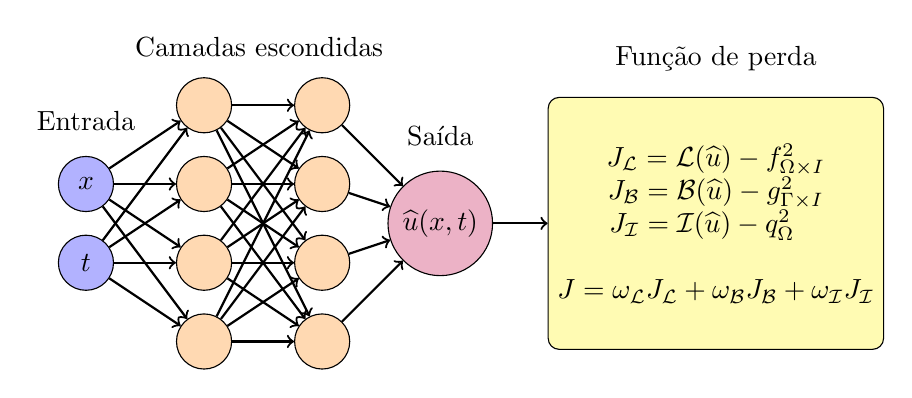
\begin{tikzpicture}[
    neuron/.style={circle, draw, minimum size=0.7cm},
    input/.style={neuron, fill=blue!30},
    hidden/.style={neuron, fill=orange!30},
    output/.style={neuron, fill=purple!30},
    physnode/.style={rectangle, draw, rounded corners, fill=orange!30, minimum width=1.5cm, minimum height=1.8cm},
    lossnode/.style={rectangle, draw, rounded corners, fill=yellow!30, minimum width=2cm, minimum height=3.2cm, align=center},
    every edge/.style={draw, ->, thick}
]

\node[input] (I-1) at (0, 2) {$x$};
\node[input] (I-2) at (0, 1) {$t$};

\node[hidden] (H1-1) at (1.5, 3) {};
\node[hidden] (H1-2) at (1.5, 2) {};
\node[hidden] (H1-3) at (1.5, 1) {};
\node[hidden] (H1-4) at (1.5, 0) {};

\node[hidden] (H2-1) at (3, 3) {};
\node[hidden] (H2-2) at (3, 2) {};
\node[hidden] (H2-3) at (3, 1) {};
\node[hidden] (H2-4) at (3, 0) {};

\node[output] (O-1) at (4.5, 1.5) {$\widehat{u}(x,t)$};

% Connections
\foreach \i in {1,2}
    \foreach \j in {1,...,4}
        \path (I-\i) edge (H1-\j);

\foreach \i in {1,...,4}
    \foreach \j in {1,...,4}
        \path (H1-\i) edge (H2-\j);

\foreach \j in {1,...,4}
    \path (H2-\j) edge (O-1);

\node[lossnode] (TotalLoss) at (8, 1.5) {
$J_{\mathcal{L}} = \lVert \mathcal{L}(\widehat{u}) - f \rVert^{2}_{\Omega \times I}$
\\
$J_{\mathcal{B}} = \lVert \mathcal{B}(\widehat{u}) - g \rVert^{2}_{\Gamma \times I}$
\\
$J_{\mathcal{I}} = \lVert \mathcal{I}(\widehat{u}) - q \rVert^{2}_{\Omega} \quad$
\\
\\
$J = \omega_{\mathcal{L}} J_{\mathcal{L}} + \omega_{\mathcal{B}} J_{\mathcal{B}} + \omega_{\mathcal{I}} J_{\mathcal{I}}$
};

\path (O-1) edge (TotalLoss);

% Labels
\node[above=0.2cm] at (I-1.north) {Entrada};
\node[above=0.2cm] at (2.2, 3.3) {Camadas escondidas};
\node[above=0.2cm] at (O-1.north) {Saída};
\node[above=0.2cm] at (TotalLoss.north) {Função de perda};

\end{tikzpicture}
\caption{Representação gráfica das PINNs. Fonte: elaborada pelos autores.}
\label{fig:pinn-representacao-grafica}
\end{figure}

A formulação acima vale tanto para problemas diretos, quanto para problemas 
inversos

\subsection{Pontos de Colocação}

Pontos de colocação são um conceito importante para as PINNs, sendo analogo
a criação da malha do \textit{MEF}. Entretanto não há um critério em que um
ponto de   

\subsection{Formulação de Problemas Inversos}

$\boldsymbol{\lambda}$

\begin{eqnarray}\label{eq:loss-total-problema-inverso} 
    \mathcal{L}_{\text{total}}(\boldsymbol{\theta}, \boldsymbol{\lambda}) 
    = \omega_{\text{física}} \mathcal{L}_{\text{física}}(\boldsymbol{\theta}, \boldsymbol{\lambda}) 
    + \omega_{\text{dados}} \,\mathcal{L}_{\text{dados}}(\boldsymbol{\theta})
\end{eqnarray}


\begin{equation}\label{eq:otimizacao-parametros-problema-inverso}
   (\boldsymbol{\theta}^*, \boldsymbol{\lambda}^*) 
   = \arg \min_{\boldsymbol{\theta}, \boldsymbol{\lambda}} \mathcal{L}_{\text{total}}(\boldsymbol{\theta}, \boldsymbol{\lambda}), 
\end{equation}

\subsection{Arquiteturas Alternativas}

A definição de PINNs como uma rede neural com informação física não se aplica
apenas a redes \textit{feedfoward}, qualquer arquitetura de redes neurais
que inclui equações que descrevem os dados em que rede está sendo treinada, pode
ser considerada uma rede neural informada pela física, uma PINN.

Desde a publicação do artigo seminal em 2019, uma série de 

\section{Modelos Compartimentais}

Baseados neste trabalho seminal,foram propostos outros modelos com mais mais 
compartimentos como o \textit{SEIRD} \cite{giles:77-sird} que inclui um 
compartimento para individuos que foram expostos a doença, mas 
ainda não manifestaram sintomas. 
Outro exemplo é o \textit{SIRV} \cite{schlickeiser-kroger:21-sirv} 
que inclui um compartimento para vacinados.

Em \cite{kendall:2023-modelos-epd-estocasticos}, é introduzido um modelo estocástico
baseado no trabalho já citado.

$R_0$ número básico

\begin{equation}
    R_0 = \frac{\beta}{\gamma}
\end{equation}

Apresentado no trabalho seminal de \cite{kermack-mcKendrick:1927}, o modelo 
\textit{SIR} é definido pelo conjunto de equações \ref{eq:SIR-1}, \ref{eq:SIR-2}
e \ref{eq:SIR-3}.

\begin{eqnarray}\label{eq:sir}
   \frac{dS(t)}{dt} &=& -\beta S(t) I(t),  \quad t > t_0, \label{eq:SIR-1}\\
   \frac{dI(t)}{dt} &=& \beta S(t) I(t) - \gamma I(t), \quad t > t_0, \label{eq:SIR-2}\\
   \frac{dR(t)}{dt} &=& \gamma I(t),  \quad t > t_0, \label{eq:SIR-3} \\
   S(t) + I(t) + R(t) &=& N,  \quad t > t_0, \label{eq:SIR-4}
\end{eqnarray}

O modelo pode ser entendido com um grafo\dots A figura \ref{fig:sir-grafo}
ilustra o modelo \textit{SIR}.

\begin{figure}
\centering
\begin{tikzpicture}[
    node distance=2.5cm,
    box/.style={rectangle, minimum width=2cm, minimum height=1.5cm, 
                draw=black, thick, align=center, rounded corners=5pt,
                font=\large\bfseries},
    arrow/.style={-Stealth, thick, line width=1.2pt},
    label/.style={midway, sloped, font=\small}
]

    % Define nodes
    \node[box, fill=blue!20] (S) {Susceptible \\ S(t)};
    \node[box, fill=red!20, right=of S] (I) {Infected \\ I(t)};
    \node[box, fill=green!20, right=of I] (R) {Recovered \\ R(t)};

    % Transitions
    \draw (S) edge[->] node[label,above] {$\beta$} (I);
    \draw (I) edge[->] node[label,above] {$\gamma$} (R);

\end{tikzpicture}
\caption{Grafo para o \textit{SIR}. Fonte: elaborada pelos autores.}
\label{fig:sir-grafo}
\end{figure}


\begin{equation}
    \mathcal{T} = \frac{\gamma}{\beta}N = \frac{N}{R_0}
\end{equation}


\begin{figure}[htpb]
\centering
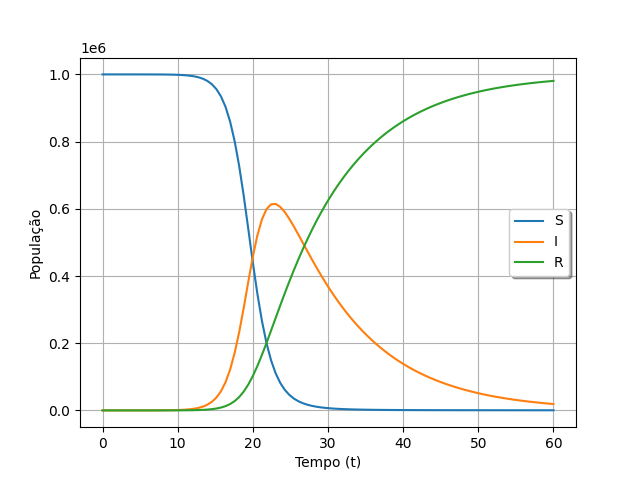
\includegraphics[width=0.6\textwidth]{figuras/sir-example-beta0.8-gamma0.1.png}
\caption{Exemplo do SIR com $\beta=0.8$ e $\gamma=0.1$.}
\label{fig:exemplo-sir}
\end{figure}

\section{Problemas Inversos}

Problemas inversos são mal-postos\dots

Identificabilidade de um modelo\dots

\section{Aplicação de PINNs com Modelos Compartimentais}

Modelos de ordem facionária \cite{li-etal:25-ordem-fracionaria}

Sir reação-difusão \cite{bertaglia-etal:22-sir-reacao-difusao}

Um exemplo utilizando redes neurais recorrentes pode ser encontrado em \cite{rodriguez-etal:2022-einns}

No artigo original, são utilizados \textit{Multi-layer Perceptrons} (MLPs)
como arquitetura das redes, mas há propostas com utilizando outras arquiteturas.
Uma proposta utilizando redes neurais convolucionais pode ser encontrada em 
\cite{shi-etal:24-convnet}. Uma proposta utilizando PINNs combinado com 
métodos Bayesianos pode ser encontrada em \cite{yang:21-bpinns}, esta 
abordagem é particulamente interessante para problemas inversos, ao transformar
a estimativa dos parâmetros numa distribuição, no lugar de um valor fixo.
